\documentclass[tikz,border=10pt,fleqn]{article}
\title{Bell's spaceship paradox}
\author{Hans Halvorson}
\date{\today}
\usepackage{pgfplots}
\pgfplotsset{compat=newest}

\usepackage{amsfonts}
\usepackage{amsthm}
\theoremstyle{definition}
\usepackage{amsthm}
\newtheorem*{question}{Question}
\newtheorem*{fact}{Fact}

\newcommand{\vecc}[1]{\overrightarrow{#1}}

\begin{document}

\maketitle

We assume that Alice (leading) and Bob (trailing) receive the
instruction to accelerate at the same time (in what was originally
their common reference frame). Bob's trajectory (blue) is given by
\[ b(t) \: = \: (\cosh (t),\sinh (t)) , \] and Alice's trajectory
(green) is given by
\[ a(t) \: = \: (\cosh (t)+1,\sinh (t)) ,\] for
$t\in\mathbb{R}^+$. Since $b(t)=(1,0)+a(t)$, we have $b'(t)=a'(t)$,
where \[ a'(t) \: = \: (\sinh (t),\cosh(t)) ,\] and
\[ a''(t) \: = \: (\cosh (t),\sinh (t)) .\] In particular,
\[ \| a''(t) \|^2 = \sinh ^2 (t)-\cosh ^2(t) = 1 ,\] for all $t$,
i.e.\ Alice and Bob have constant acceleration.

In the following diagram, the red vector is tangent to Bob's
trajectory at the point $(\sqrt{2},1)$. The dashed blue line is Bob's
orthogonal spacelike hypersurface when he is located at
$(\sqrt{2},1)$, and the dashed green line is Alice's orthogonal
spacelike hypersurface when she is located at $(\sqrt{2}+1,1)$.

\bigskip \noindent 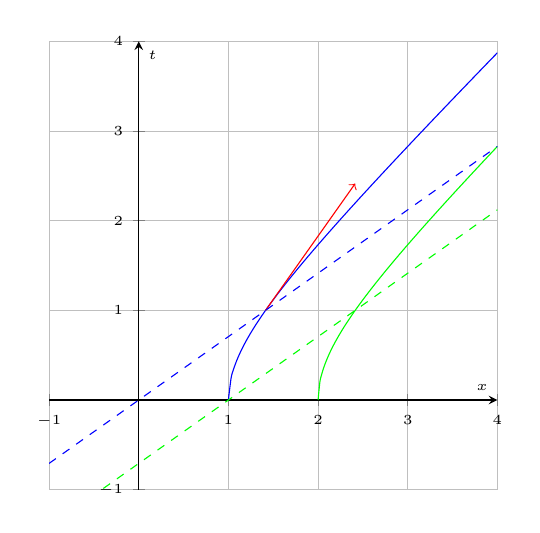
\begin{tikzpicture}
    \begin{axis}[
        axis lines=middle,
        xlabel={$x$},
        ylabel={$t$},
        xlabel style={font=\tiny}, % Makes the x-axis label smaller
        ylabel style={font=\tiny}, 
        xmin=-1, xmax=4,
        ymin=-1, ymax=4,
        grid=both,
        grid style={line width=.1pt, draw=gray!10},
        major grid style={line width=.2pt,draw=gray!50},
        axis equal image,
        legend pos=north west,
        tick label style={font=\tiny}, 
    ]
    % Original hyperbola (positive y values only)
    \addplot[domain=1:4, samples=100, smooth, blue] {sqrt(x^2 - 1)};

    % Shifted hyperbola (positive y values only)
    \addplot[domain=2:4, samples=100, smooth, green] {sqrt((x-1)^2 - 1)};

    % Tangent vector at x=2
    \draw[->, red] (axis cs:{sqrt(2)},1)--++(axis direction cs:1,{sqrt(2)});

    % Calculate slope
    \pgfmathsetmacro{\slope}{1/sqrt(2)}

    % Calculate y-intercept
    \pgfmathsetmacro{\yintercept}{1 - \slope*sqrt(2)}

    % Plot the line
    \draw[blue, dashed] (-1,{\slope*-1 + \yintercept}) -- (4,{\slope*4 + \yintercept}) node[right] {};

    \pgfmathsetmacro{\yinterceptNew}{1 - \slope*(1 + sqrt(2))}

    % Plot the new line
    \draw[green, dashed] (-1,{\slope*-1 + \yinterceptNew}) -- (4,{\slope*4 + \yinterceptNew}) node[right] { };
    \end{axis}
  \end{tikzpicture}

  \bigskip \noindent Each each time $t$, Alice and Bob have the same
  tangent vector, and so they foliate Minkowski spacetime into the
  same family of spatial hypersurfaces. However, Alice and Bob are
  located on different timeslices of the relevant foliation. For
  example, Bob reaches coordinate $(\sqrt{2},1)$ in the lab frame at
  the same time that Alice reaches coordinate
  $(1+\sqrt{2},1)$. [Alice's trajectory results from translating Bob's
  trajectory by the vector $\vecc{b(0)a(0)}$.]  At this time, their
  common foliation consists of lines with slope $1/\sqrt{2}$, but Bob
  lies on the line that has $y$-intercept $0$, while Alice lies on the
  line that has $y$-intercept $-1/\sqrt{2}$.

  \begin{fact} The spacetime distance between Alice and Bob does not
    change. To be more precise, if $a(t)$ represents Alice's position
    at time $t$ and $b(t)$ represents Bob's position at time $t$, then
    $\vecc{b(t)a(t)}$ is a spacelike vector and
    $\| \vecc{b(t)a(t)} \|=1$. \end{fact}

This follows directly from the fact that Alice's trajectory is simply
a constant shift of Bob's trajectory.

\begin{fact} The point $(1,0)=b(0)$ lies on Alice's simultaneity
  surface for all $t\in\mathbb{R}^+$. What's more, $\vecc{b(0)a(t)}$
  is spacelike, and $\| \vecc{b(0)a(t)}\| =1$ for all
  $t\in\mathbb{R}^+$. \end{fact}

\begin{proof} The hyperbola
  $\{ (\cosh (t),\sinh(t)):t\in\mathbb{R} \}$ consists of points that
  are Minkowski distance $1$ from $(0,0)$. Hence the hyperbola
  $\{ (\cosh (t)+1,\sinh (t)):t\in\mathbb{R}\}$ consists of points
  that are Minkowski distance $1$ from $(1,0)$.
\end{proof}


\begin{question} What is the orthogonal (temporal) distance between
  Alice and Bob's hypersurfaces at time $t$? Conjecture: it is the
  same as the length of the tangent vector $v(t)$. To see this, just
  do the pythagorean theorem with the triangle where $v(t)$ is the
  hypotenuse. \end{question}

\begin{question} What's does Alice's motion look like to Bob? What
  does Bob's motion look like to Alice? \end{question}

\begin{question} What is the distance, in Bob's frame, between Bob and
  Alice? \end{question}

\begin{question} Show that $\| a'(t)\|$ is bounded in
  length. \end{question}   
\end{document}


%%% Local Variables:
%%% mode: latex
%%% TeX-master: t
%%% End:
